\documentclass[a4paper,11pt,times]{article}

\usepackage[czech]{babel}
\usepackage[utf8]{inputenc}

\usepackage{natbib}
\usepackage{graphicx}
\usepackage{ragged2e}
\usepackage{geometry}
\usepackage{setspace}
\usepackage[czech,linesnumbered,ruled,noline]{algorithm2e}
\usepackage{url}
\usepackage{hyperref}
\usepackage{multirow}\usepackage{multicol}
\usepackage{pdflscape}

 \geometry{
 a4paper,
 text={170mm,240mm},
 left=20mm,
 top=30mm,
 }
 
 \urlstyle{same}
 
 %konec hlavicky

\begin{document}


\begin{titlepage}
\begin{justify}
\Huge

\centering{\textsc{{{Vysoké učení technické v Brně \\ \huge{Fakulta informačních technologií}\\}}}}
\end{justify}
\vspace{\stretch{0.382}}
\begin{center}
\large
\textbf{\setstretch{0.3}{
Typografie a publikování – 3. projekt\\[0.4em]
\LARGE
Tabulky a obrázky\\
\vspace{\stretch{0.618}}}}
\end{center}

\Large
{\LARGE \today \hfill Jan Zbořil (xzbori20)}
\end{titlepage}

\section{Úvodní strana}
Název práce umístěte do zlatého řezu a nezapomeňte uvést dnešní datum a vaše jméno a příjmení.

\section{Tabulky}
Pro sázení tabulek můžeme použít buď prostředí \verb tabbing  nebo prostředí \verb tabular  .

\subsection{Prostředí \texttt{tabbing}}
Při použití \verb tabbing  vypadá tabulka následovně:

\begin{tabbing}
    Ovoce \hspace{2cm} \= Cena \hspace{0.5cm} \= Množství \\
    Jablka \> 25,90 \> 3 kg \\
    Hrušky \> 27,40 \> 2,5 kg \\
    Vodní melouny \> 35,- \> 1 kus
\end{tabbing}

\noindent
Toto prostředí se dá také použít pro sázení algoritmů, ovšem vhodnější je použít prostředí \verb algorithm  nebo \verb algorithm2e  (viz sekce \ref{algoritmy}).

\subsection{Prostředí \texttt{tabular}}
Další možností, jak vytvořit tabulku, je použít prostředí \verb tabular . Tabulky pak budou vypadat takto\footnote{Kdyby byl problem s \texttt{cline} , zkuste se podívat třeba sem: \url{http://www.abclinuxu.cz/tex/poradna/show/325037}}:

\begin{table}[ht] \catcode`\-=12
\begin{center}
\begin{tabular}{| c | c | c |}
    \hline
    \multirow{2}{*}{\textbf{Měna}} & \multicolumn{2}{c|}{\textbf{Cena}} \\
    \cline{2-3}
    & \textbf{nákup} & \textbf{prodej} \\
    \hline
    EUR & 25,475 & 27,045 \\ 
    GBP & 28,835 & 30,705 \\
    USD & 22,943 & 24,357 \\
    \hline
\end{tabular}
    \caption{Tabulka kurzů k dnešnímu dni}
    \label{table_kurz}
\end{center}
\end{table}

\begin{table}[ht] \catcode`\-=12
\begin{center}
\begin{tabular}{| c | c |}
    \hline
    $A$ & $\neg A$ \\
    \hline
    \textbf{P} & P \\
    \hline
    \textbf{O} & O \\
    \hline
    \textbf{X} & X \\
    \hline
    \textbf{N} & N \\
    \hline
\end{tabular}
\begin{tabular}{| c | c | c | c | c | c |}
    \hline
    \multicolumn{2}{| c}{\multirow{2}{*}{$A \land B$}} & \multicolumn{4}{| c |}{B} \\
    \cline{3-6}
    \multicolumn{2}{| c |}{} & \textbf{P} & \textbf{O} & \textbf{X} & \textbf{N} \\
    \hline
    \multirow{4}{*}{$A$} & \textbf{P} & P & O & X & N \\
    \cline{2-6}
     & \textbf{O} & O & O & N & N \\
    \cline{2-6}
     & \textbf{X} & X & N & X & N \\
    \cline{2-6}
     & \textbf{N} & N & N & N & N \\
    \hline
\end{tabular}
\begin{tabular}{| c | c | c | c | c | c |}
    \hline
    \multicolumn{2}{| c}{\multirow{2}{*}{$A \lor B$}} & \multicolumn{4}{| c |}{B} \\
    \cline{3-6}
    \multicolumn{2}{| c |}{} & \textbf{P} & \textbf{O} & \textbf{X} & \textbf{N} \\
    \hline
    \multirow{4}{*}{$A$} & \textbf{P} & P & P & P & P \\
    \cline{2-6}
     & \textbf{O} & P & O & P & O \\
    \cline{2-6}
     & \textbf{X} & P & P & X & X \\
    \cline{2-6}
     & \textbf{N} & P & O & X & N \\
    \hline
\end{tabular}
\begin{tabular}{| c | c | c | c | c | c |}
    \hline
    \multicolumn{2}{| c}{\multirow{2}{*}{$A \to B$}} & \multicolumn{4}{| c |}{B} \\
    \cline{3-6}
    \multicolumn{2}{| c |}{} & \textbf{P} & \textbf{O} & \textbf{X} & \textbf{N} \\
    \hline
    \multirow{4}{*}{$A$} & \textbf{P} & P & O & X & N \\
    \cline{2-6}
     & \textbf{O} & P & O & P & O \\
    \cline{2-6}
     & \textbf{X} & P & P & X & X \\
    \cline{2-6}
     & \textbf{N} & P & P & P & P \\
    \hline
\end{tabular}
    \caption{Protože Kleeneho trojhodnotová logika už je \uv{zastaralá}, uvádíme si zde příklad čtyřhodnotové logiky}
    \label{table_Kleen}
\end{center}
\end{table}

\newpage
\section{Algoritmy}\label{algoritmy}
Pokud budeme chtít vysázet algoritmus, můžeme použít prostředí \verb algorithm \footnote{Pro nápovědu, jak zacházet s prostředím \texttt{algorithm}, můžezeme zkusit tuhle stránku:
\newline \url{http://ftp.cstug.cz/pub/tex/CTAN/macros/latex/contrib/algorithms/algorithms.pdf}.} nebo \verb algorithm2e \footnote{Pro \texttt{algorithm2e} zase tuhle: \href{http://ftp.cstug.cz/pub/tex/CTAN/macros/latex/contrib/algorithm2e/doc/algorithm2e.pdf}{http://ftp.cstug.cz/pub/tex/CTAN/macros/latex/contrib/algorithm2e/doc/algorithm2e.pdf}.}. Příklad použití prostředí \verb algorithm2e  viz Algoritmus \ref{Algortimus 1}.

\begin{algorithm}
\label{Algortimus 1}
\caption{\textsc{FastSlam}}
\SetKwData{Left}{left}\SetKwData{This}{this}\SetKwData{Up}{up}
\SetKwFunction{Union}{Union}\SetKwFunction{FindCompress}{FindCompress}
\SetKwInOut{Input}{Input}\SetKwInOut{Output}{Output}
    \Input{$(X_{t-1},u_t,z_t)$}
    \Output{$X_t$}
        \BlankLine
        \IncMargin{2cm}
        $ \overline{X_t} = X_t = 0$ \\
        \For{$k = 1$ \KwTo $M$}{
            $x_t^{[k]}$ = \emph sample\_motion\_model$(u_t,x_{t-1}^{[k]})$ \\
            $\omega_t^{[k]}$ = \emph measurement\_model$(z_t,x_{t}^{[k]},m_{t-1})$ \\
            $m_t^{[k]}$ = \emph updated\_occupancy\-grid$(z_t,x_{t}^{[k]},m_{t-1}^{[k]})$ \\
            $ \overline{X_t} = \overline{X_t} + \langle x_x^{[m]},\omega_x^{[m]} \rangle$ \\
        }
        \For{$k = 1$ \KwTo $M$}{
            draw $i$ with probability $\approx \omega_t^{[i]}$ \\
            add $\langle x_x^{[k]},m_t^{[k]} \rangle$ to $X_t$\\
        }
        \Return $X_t$
        
\end{algorithm}

\section{Obrázky}
Do našich článků můžeme samozřejmě vkládat obrázky. Pokud je obrázkem fotografie, můžeme klidně použít bitmapový soubor. Pokud by to ale mělo být nějaké schéma nebo něco podobného, je dobrým zvykem takovýto obrázek vytvořit vektorově.

\begin{figure}[ht]
    \centering
    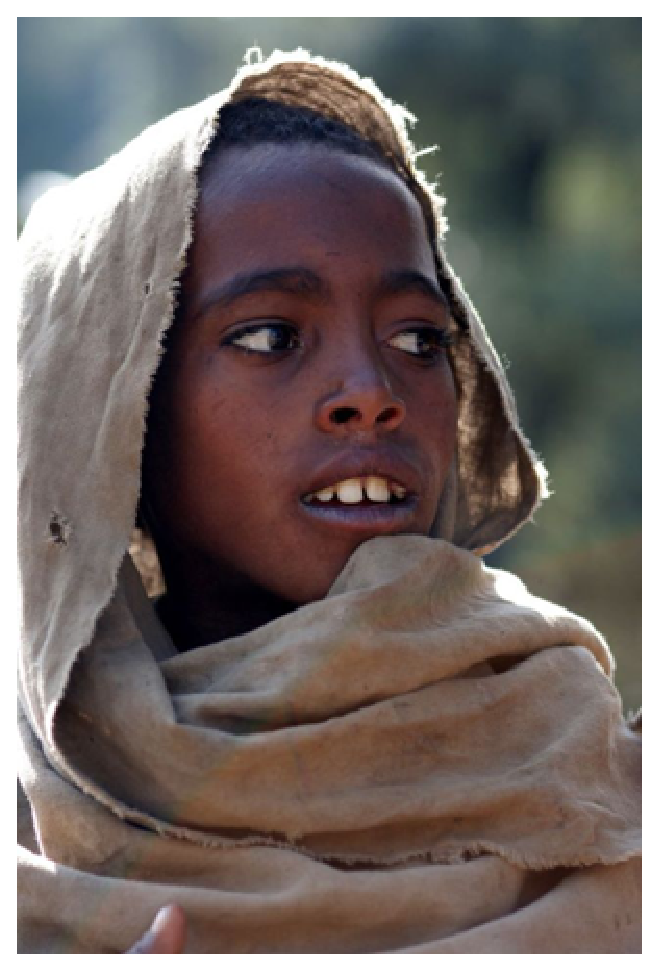
\includegraphics[scale=0.4]{etiopan.eps}
    \scalebox{-0.4}[0.4]{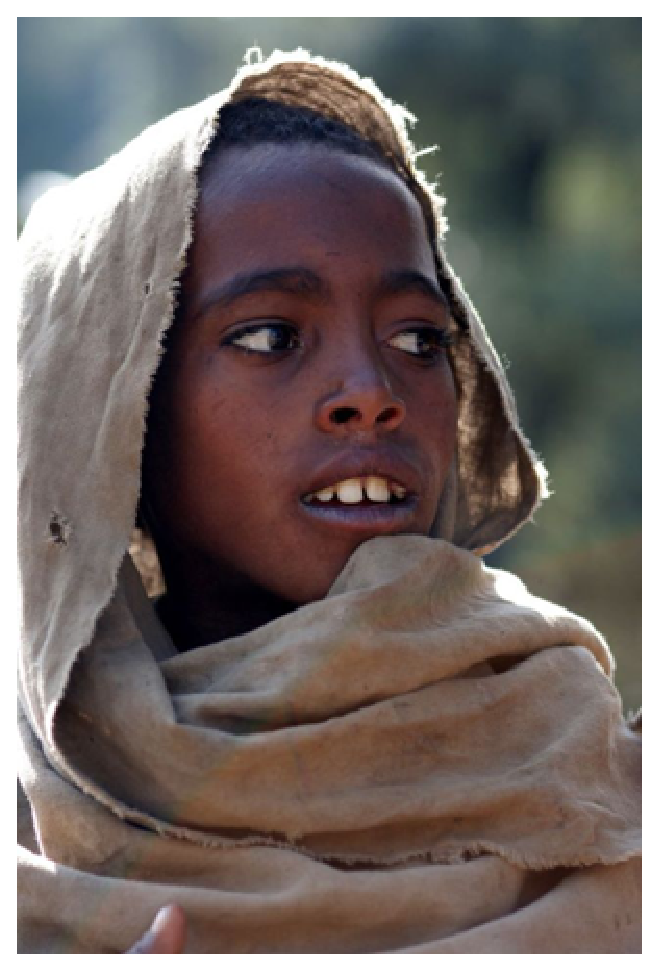
\includegraphics[]{etiopan.eps}} \\
    \caption{Malý Etiopánek a jeho bratříček}
    \label{obr1}
\end{figure}

\newpage

Rozdíl mezi vektorovým...
\begin{figure}[ht]
    \centering
    
\includegraphics[scale=0.4]{oniisan.eps}
    \caption{Vektorový obrázek}
    \label{ob2}
\end{figure}
\\
... a bitmapovým obrázkem
\begin{figure}[ht]
    \centering
    
\includegraphics[scale=0.6]{oniisan2.eps}
    \caption{Bitmapový obrázek}
    \label{ob3}
\end{figure}
\\
se projeví například po zvětšení.

Odkazy (nejen ty) na obrázky \ref{obr1}, \ref{ob2} a \ref{ob3}, na tabulky \ref{table_kurz} a \ref{table_Kleen} a také na algoritmus \ref{Algortimus 1} jsou udělány pomocí křížových odkazů. Pak je ovšem potřeba zdrojový soubor přeložit dvakrát. 
Vektorové obrázky lze vytvořit i přímo v \LaTeX u, například pomocí prostředí \verb picture .

\newpage
\centering
\begin{landscape}
\setlength{\unitlength}{1cm}
\thicklines
\begin{figure}
    \centering
    \begin{picture}(20,15)
    \put(0,0){\line(1,0){20}}
    \put(0,15){\line(1,0){20}}
    \put(0,0){\line(0,1){15}}
    \put(20,0){\line(0,1){15}}
    
    \put(17,13){\circle{2}}
    \put(2,2){\linethickness{0.2cm}\line(1,0){16}}
    
    \put(3,2){\linethickness{0.1cm}\line(0,1){8}}
    \put(7,2){\linethickness{0.1cm}\line(0,1){8}}
    \put(3,10){\linethickness{0.1cm}\line(1,0){1}}
    \put(6,10){\linethickness{0.1cm}\line(1,0){1}}
    \put(4,9){\linethickness{0.1cm}\line(1,0){2}}
    \put(4,9){\linethickness{0.1cm}\line(0,1){1}}
    \put(6,9){\linethickness{0.1cm}\line(0,1){1}}
    \put(3.5,10){\linethickness{0.5cm}\line(1,2){1.5}}
    \put(6.5,10){\linethickness{0.2cm}\line(-1,2){1.5}}
    \put(5,13){\circle*{1}}
    \put(5,6){\oval(1,3)[tl]}\put(5,6){\oval(1,3)[tr]}
    \put(4,6){\line(1,0){2}}
    
    \put(13,2){\linethickness{0.1cm}\line(0,1){8}}
    \put(17,2){\linethickness{0.1cm}\line(0,1){8}}
    \put(16,10){\linethickness{0.1cm}\line(1,0){1}}
    \put(13,10){\linethickness{0.1cm}\line(1,0){1}}
    \put(14,9){\linethickness{0.1cm}\line(1,0){2}}
    \put(14,9){\linethickness{0.1cm}\line(0,1){1}}
    \put(16,9){\linethickness{0.1cm}\line(0,1){1}}
    \put(13.5,10){\linethickness{0.5cm}\line(1,2){1.5}}
    \put(16.5,10){\linethickness{0.2cm}\line(-1,2){1.5}}
    \put(15,13){\circle*{1}}
    \put(15,6){\oval(1,3)[tl]}\put(15,6){\oval(1,3)[tr]}
    \put(14,6){\line(1,0){2}}
    
    \put(7,8){\linethickness{0.1cm}\line(1,0){6}}
    \put(7,8){\linethickness{0.1cm}\line(1,1){3}}
    \put(13,8){\linethickness{0.1cm}\line(-1,1){3}}
    \put(10,11){\circle*{1}}
    
    \put(10,5){\oval(2,3)[tl]}
    \put(10,5){\oval(2,3)[tr]}
    \put(10,2){\linethickness{0.1cm}\line(0,1){4.5}}
    \put(9,2){\linethickness{0.1cm}\line(0,1){3.5}}
    \put(11,2){\linethickness{0.1cm}\line(0,1){3.5}}
    \put(10,2){\linethickness{0.1cm}\line(1,1){1}}
    \put(10,3){\linethickness{0.1cm}\line(1,1){1}}
    \put(10,4){\linethickness{0.1cm}\line(1,1){1}}
    \put(10,5){\linethickness{0.1cm}\line(1,1){1}}
    \put(10,6){\linethickness{0.1cm}\line(1,1){0.5}}
    \put(10,2){\linethickness{0.1cm}\line(-1,1){1}}
    \put(10,3){\linethickness{0.1cm}\line(-1,1){1}}
    \put(10,4){\linethickness{0.1cm}\line(-1,1){1}}
    \put(10,5){\linethickness{0.1cm}\line(-1,1){1}}
    \put(10,6){\linethickness{0.1cm}\line(-1,1){0.5}}
    
    \end{picture}
    \caption{To je ale pěkný hrad - Vektorštejn.}
\end{figure}

\end{landscape}
\end{document}
